\subsection{Teilaufgabe 1: Algorithmik}

\subsection{Teilaufgabe 2: Theoretische Informatik}

\subsubsection{Aufgabe 1: Reguläre Sprachen}

\begin{teile}
	\item
		 
	$DEA = (\{ 1,2,3,4\},\{ a,b,c\},\delta,1,\{ 1,2\})$, wobei $\delta$ gegeben ist durch:
		
	\begin{tabular}{c|ccc}
		Zustand & a & b & c \\
		\hline
		1       & 2 & 1 & 1 \\
		2       & 3 & 1 & 1 \\
		3       & 4 & 1 & 4 \\
		4       & 4 & 4 & 4 \\
	\end{tabular} 
		
	Grafische Darstellung:
	\begin{center}
		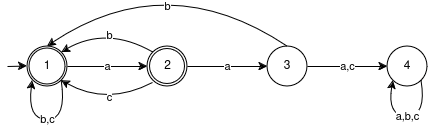
\includegraphics[scale=0.9]{DEA.png}
	\end{center}	
			
	\item
	Die Anzahl der Äquivalenzklassen kann die Anzahl an Zuständen nicht überschreiten, die der DEA aufweist, welcher diese Sprache erkennt. Der DEA aus a) verfügt über vier Zustände, also hat $L_1$ maximal vier Äquivalenzklassen.

	Wir finden vier unterschiedliche Äquivalenzklassen zu den Repräsentanten $\varepsilon, a, aa$ und $aaa$:
	\begin{itemize}
		\item Da $\varepsilon \circ a \in L_1$, aber $a \circ a \notin L_1$ gilt $[\varepsilon]\nsim_{L_1}[a]$.
		\item Da $\varepsilon \circ a \in L_1$, aber $aa \circ a \notin L_1$ gilt $[\varepsilon]\nsim_{L_1}[aa]$.
		\item Da $\varepsilon \circ a \in L_1$, aber $aaa \circ a \notin L_1$ gilt $[\varepsilon]\nsim_{L_1}[aaa]$.
		\item Da $a \circ c \in L_1$, aber $aa \circ c \notin L_1$ gilt $[a]\nsim_{L_1}[aa]$.
		\item Da $a \circ c \in L_1$, aber $aaa \circ c \notin L_1$ gilt $[a]\nsim_{L_1}[aaa]$.
		\item Da $aa \circ b \in L_1$, aber $aaa \circ b \notin L_1$ gilt $[aa]\nsim_{L_1}[aaa]$.
	\end{itemize}
	
	Drei Wörter je Äquivalenzklasse:
	\begin{enumerate}
		\item $bc, ccc, bbb \in [\varepsilon]$
		\item $a, aca, aba \in [a]$
		\item $aa, aabaa, abaa \in [aa]$
		\item $aaa, aac, aaabc \in [aaa]$
	\end{enumerate}
	\vspace{0.3cm}
	
	%\newpage
	\item 
	\textbf{Übergangstabelle}
	
	\begin{tabular}{|c|c|c|c|}
		\hline
		\textbf{Zustand}  & \textbf{a-Übergang} & \textbf{b-Übergang} & \textbf{$\epsilon$-Übergang} \\
		\hline
		1                 & 2                   & 1                   & 4 \\
		\hline
		2                 & 3                   & $\varnothing$       & $\varnothing$ \\
		\hline
		3                 & 1                   & 2                   & 1 \\
		\hline
		4                 & $\varnothing$       & 3                   & $\varnothing$ \\
		\hline
	\end{tabular}
	
	
	\textbf{$\epsilon$-Funktionsabschlusstabelle}
		
	\begin{tabular}{|c|c|}
		\hline
		\textbf{Zustand}  & \textbf{Funktionsabschluss} \\
		\hline
		1                 & \{1,4\} \\
		\hline
		2                 & \{2\} \\
		\hline
		3                 & \{1,3,4\}  \\
		\hline
		4                 & \{4\} \\
		\hline
	\end{tabular}
	
	\textbf{Pontenzmengenkonstruktionstabelle}
	
	\begin{tabular}{|c|c|c|c|}
		\hline
		\textbf{Zustand} & \textbf{a-Übergang} & \textbf{b-Übergang} & \textbf{Endzustand?} \\
		\hline
		\{1,4\}     & \{2\}       & \{1,3,4\}         & Ja \\
		\hline
		\{2\}       & \{1,3,4\}   & \{$\varnothing$\} &    \\
		\hline
		\{1,3,4\}   & \{1,2,4\}   & \{1,2,3,4\}       & Ja \\
		\hline
		\{1,2,4\}   & \{1,2,3,4\} & \{1,3,4\}         & Ja \\
		\hline
		\{1,2,3,4\} & \{1,2,3,4\} & \{1,2,3,4\}       & Ja \\
		\hline
		\{$\varnothing$\}       & \{$\varnothing$\}   & \{$\varnothing$\} &    \\
		\hline
	\end{tabular}	
	
	\textbf{Fertiger DEA} \\
	
	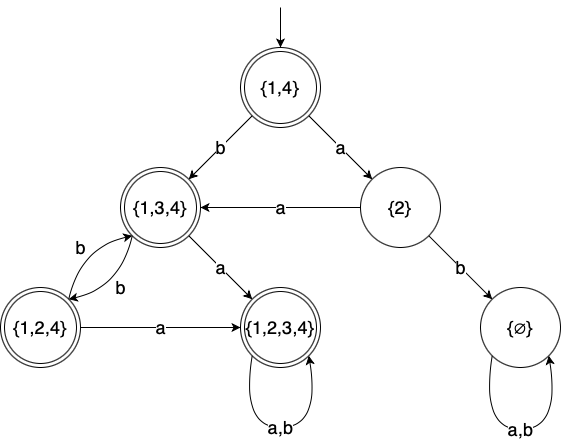
\includegraphics[scale=0.5]{NEA-DEA}
	
\end{teile}

\newpage
\subsubsection{Aufgabe 2: Regularität und Kontextfreiheit}

\begin{teile}
	\item
	$L_1 = \{a^mb^nc^n \mid n,m \geq 1; n,m \in \mathbb{N} \} \cup \{ b^m c^n \mid n,m \geq 0; n,m \in \mathbb{N}\}$	
	
	\begin{quote}
	\textbf{Pumpinglemma für reguläre Sprachen} \\
    Ist $L_1$ regulär, so gilt: \\
    $\exists p \geq 1: \forall z \in L, |z| \geq p:$ \\
    $\exists u,v,w \in \Sigma^*: z = uvw$ mit
    \begin{enumerate}
    	\item $|v|  \geq 1$
    	\item $|uv| \leq p$
    	\item $\forall i \in \mathbb{N} : uv^{i}w \in L_1$
    \end{enumerate}
	\end{quote}
	
	%Betrachten wir zunächst $L_2 := L_1\ \cap\ aa^*b^*c^*$ und nehmen an $L_2$ sei regulär.
	Nehmen wir an $L_1$ sei regulär, dann können wir das Pumpinglemma anwenden und folgern:
	
	Sei $p \geq 1$ die Pumpingzahl. Wir wählen $z = ab^pc^p \in L_1$ mit $|z| = 2p+1 \geq p$.\\
	Aus $|uv| \leq p$ folgt: $uv$ ist von der Form $ab^{p-n}$ für ein $n \in \{1,2,...,p\}$ und $w$ ist von der Form $b^nc^p$.\\
	Aus $|v|  \geq 1$ folgt: $v$ ist von der Form $ab^k$ oder $b^{k+1}$ mit $k \in \{0,1,...,p-n\}$.\\
	Im Fall $v=ab^k$ ist $uv^0w=b^{p-k}c^p \notin L_1$, da $m=0$.\\
	Im Fall $v=b^{k+1}$ ist $uv^0w=ab^{p-k-1}c^p \notin L_1$, da $p-k-1\neq p$.
	
	Das ist ein Widerspruch zur Annahme $L_1$ sei regulär. $\Rightarrow L_1$ ist nicht regulär!
    
    %Die erste Vereinigungsmenge von $L_1$ ist also nicht regulär. Von der zweiten könnten wir zeigen, dass sie regulär ist, indem wir einen DEA für sie angeben. Da aber die Vereinigung einer regulären Sprache mit einer kontextfreien Sprache niemals regulär sein kann, ist auch $L_1$ nicht regulär.
    \vspace{0.3cm}
	
	\item
	$L_2$ ist regulär und wird von folgendem regulären Ausdruck erzeugt: $abc(abc)^* = (abc)^+$

	Das lässt sich begründen, indem man sich die Reihenfolge der Buchstaben ansieht. $L_2$ ist so definiert, dass jedes Wort in der Sprache mit $a$ beginnen muss, darauf folgt ein $b$ und dann ein $c$, worauf wieder nur ein $a$ fogen kann u.s.w.. Zudem muss jedes Wort auf ein $c$ enden und mindestens einmal die Kombination $abc$ enthalten (der Rest fällt durch $n=0$ weg).
	
	%Michael: Man beachte, dass die mehreren gleichnamigen Zeichenwiederholungsexponenten eine fiese Blendgranate darstellen, die die Aufgabenstellung wirft, um einen zu einem Nichtregularitätsbeweis mittels Pumplemma oder Myhill-Nerode zu verlocken.
	
	% $L_2 = \{(abc)^nab(cab)^nc(abc)^n \mid n \geq 0; n \in \mathbb{N} \}$		
	% 
	% Nichtregularitätsbeweis mit Myhill-Nerode:
	% \begin{quote}
	% Sei $L_2$ eine formale Sprache. \\
	% Die binäre Relation $\sim_L \subseteq \Sigma^*$ ist gegeben durch: \\
	% $x \sim_{L_2} y :\Leftrightarrow \forall w \in \Sigma^*: xw \in L \Leftrightarrow yw \in L_2$. \\
	% Ist $L_2$ regulär, dann ist der Index von $\sim_{L_2}$ endlich.	
	% \end{quote}
	% Betrachte die Wörter $(abc)^n ab(cab)^n c$ und $(abc)^k ab(cab)^k c$ mit $k < n$. \\
	% Hängt man daran das Wort $(abc)^n$, gilt: \\
	% $(abc)^n ab(cab)^n \textcolor{red}{(abc)^n} \in L_2 \forall n \in \mathbb{N}$ \\
	% $(abc)^k ab(cab)^k \textcolor{red}{(abc)^n} \notin L_2 \forall n \in \mathbb{N}$, denn $k < n$
	% 
	% Durch paarweise gleichmäßiges Erhöhen des Zeichenwiederholungsexponenten erhält man somit unendlich viele Wörter, die sich alle paarweise nicht in derselben Äquivalenzklasse befinden.
	% 
	% $\Rightarrow \mid \sim_{L_2} \mid = \infty$ \\ 
	% $\Rightarrow L_2$ ist nicht regulär. \\

	\vspace{0.3cm}

	\item
	Als Nachweis für die Kontextfreiheit geben wir eine kontextfreie Grammatik an, die $L_3$ erzeugt:
	
	\begin{tabular}{lcl}
		S  & $\rightarrow$ & ASE $\mid$ T $\mid$ abTde \\
		T  & $\rightarrow$ & BTD $\mid$ c \\
		A & $\rightarrow$ & aa \\
		B & $\rightarrow$ & bb \\
		E  & $\rightarrow$ & ee \\
		D  & $\rightarrow$ & dd \\
	\end{tabular}
	
	\textbf{Erklärung}: \\
	Die Geradheit der Summe wird durch die Ableitungsregeln mit Doppel-Terminalen auf der rechten Seite gewährleistet. Somit können bei jeder Regel (außer für $c$) nur 2 Buchstaben pro Seite dazu kommen und die SUmme ist insgesamt immer ein Vielfaches von 2, also gerade.\\
	Der Fall, dass die A's, B's und somit auch die D's, E's jeweils eine ungerade Anzahl haben, wird durch die Regel $S \rightarrow abTde$ abgedeckt.
	\vspace{0.3cm}
	
	\item
	$L_4 = \{w_1c^nw_2 \mid n \geq 0, n \in \mathbb{N}, w_1,w_2 \in \{a,b\}^*, \#_a(w_1)>n\ und\ \#_b(w_2)<n\}$	

	\begin{quote}
	\textbf{Pumpinglemma für kontextfreie Sprachen} \\
	Ist $L_4$ eine kontextfreie Sprache, so gilt: \\
	$\exists p \in \mathbb{N}: \forall z \in L, |z| \geq p:$ \\
	$\exists u,v,w,x,y \in \Sigma^*: z = uvwxy$ mit
	\begin{enumerate}
		\item $|vx| \geq 1$
		\item $|vwx| \leq p$
		\item $\forall i \in \mathbb{N} : uv^{i}wx^{i}y \in L_4$
	\end{enumerate}
	\end{quote}

	Nehmen wir an $L_4$ sei kontextfrei, dann können wir das Pumpinglemma anwenden und folgern:
	
	Sei $p \in \mathbb{N}$ die Pumpingzahl. Wir wählen $z = a^{p+1}c^pb^{p-1} \in L_4$ mit $|z| = 3p > p$.\\
	Aus $|vwx| \leq p$ folgt: $vwx$ kann nicht aus a's, c's und b's bestehen. Die Form von $vwx$ entspricht also einem der beiden Fälle:
	\begin{enumerate}
		\item $a^ic^j$ für $i \in \{1,2,...,p+1\}$ und $j \in \{1,2,...,p\}$ mit $i+j \leq p$
		\item $c^ib^j$ für $i \in \{1,2,...,p\}$ und $j \in \{1,2,...,p-1\}$ mit $i+j \leq p$
	\end{enumerate}
	Aus $|vx| \geq 1$ ergeben sich dann für $v$ und $x$ folgende Fälle (mit $k+l+m  \geq 1$):
	\begin{itemize}
		\item Fall 1.1: $v=a^kc^l$ und $x=c^m$
		\item Fall 1.2: $v=a^k$ und $x=a^lc^m$
		\item Fall 2.1: $v=c^kb^l$ und $x=b^m$
		\item Fall 2.2: $v=c^k$ und $x=c^lb^m$
	\end{itemize}
	In Fall 1.1 ist $uv^0wx^0y=a^{p+1-k}c^{p-l-m}b^{p-1} \notin L_4$, da entweder $p-l-m \ngtr p-1$ oder falls $l=m=0:\ k\geq 1 \Rightarrow p+1-k \ngtr p-l-m$ gilt.\\
	In Fall 1.2 ist $uv^0wx^0y=a^{p+1-k-l}c^{p-m}b^{p-1} \notin L_4$, da entweder $p-m \ngtr p-1$ oder falls $m=0:\ k+l\geq 1 \Rightarrow p+1-k-l \ngtr p-m$ gilt.\\
	In Fall 2.1 ist $uv^2wx^2y=a^{p+1}c^{p+k}b^{p-1+l+m} \notin L_4$, da entweder $p+1 \ngtr p+k$ oder falls $k=0:\ l+m\geq 1 \Rightarrow p+k \ngtr p-1+l+m$ gilt.\\
	In Fall 2.2 ist $uv^2wx^2y=a^{p+1}c^{p+k+l}b^{p-1+m} \notin L_4$, da entweder $p+1 \ngtr p+k+l$ oder falls $k=l=0:\ m\geq 1 \Rightarrow p+k+l \ngtr p-1+m$ gilt.
	
	Das ist ein Widerspruch zur Annahme $L_4$ sei kontextfrei. $\Rightarrow L_4$ ist nicht kontextfrei!
	
\end{teile}


\newpage
\subsubsection{Aufgabe 3: Entscheidbarkeit}
\begin{teile}
	\item
	$L_1 - L_2 = \{ w \in L_1 \vert w \notin L_2\}$ Es handelt sich bei $L_1 - L_2$ also um die Sprache aller Wörter aus $L_1$, die in $L_2$ nicht enthalten sind.

	Das Wortproblem für reguläre Sprachen ist entscheidbar (z.B. durch einen entsprechenden DEA) und zwar in $O(n)$, da die Eingabe lediglich einmal abgelaufen werden muss. Der CYK-Algorithmus liefert den Nachweis, dass auch das Wortproblem für kontextfreie Grammatiken mit einer Zeitkomplexität von $O(n^3)$ entscheidbar ist. Somit sind also $L_1$ und $L_2$ von einer deterministische Turingmaschine (DTM) in polynomieller Zeit entscheidbar.
	
	Wir können also eine DTM bauen, die folgendermaßen funktioniert:
	\begin{itemize}
		\item
		Prüfe in polynomieller Zeit, ob die Eingabe ein Wort in $L_1$ ist.
		\item 
		Falls diese Prüfung zutreffend war, prüfe weiter, ob die Eingabe ein Wort in $L_2$ ist. Auch das erfolgt nach der vorherigen Begründung in polynomieller Zeit.
		\item
		Ergab die erste Prüfung $wahr$ und die zweite Prüfung $falsch$, ist die Eingab ein Wort in $L$. Diese Fallunterschiedung ist problemlos in konstanter Zeit feststellbar.
	\end{itemize}
	
	Die Sprache $L_1 - L_2$ kann somit durch eine DTM in polynomieller Zeit ($O(n)+O(n^3)+O(1)=O(n^3)$) entschieden werden, also liegt $L_1 - L_2$ in $\mathcal{P}$.
	
	\item
	$L \cup \overline{L} = L \cup (\Sigma^*\setminus L) = \Sigma^*$\\
	Also ist $L \cup \overline{L}$ die Sprache \textit{aller} Wörter. Diese Sprache ist regulär und somit entscheidbar.\\
	$L \cap \overline{L} = L \cap (\Sigma^*\setminus L) = \varnothing $\\
	Also ist $L \cap \overline{L}$ die \textit{leere} Sprache. Auch diese Sprache ist regulär und somit entscheidbar.

	Somit sind $L \cap \overline{L}$ und $L \cup \overline{L}$ für alle Sprachen $L$ entscheidbar, also insbesondere auch wenn $L$ semi-entscheidbar ist.

	\item
	Da $L$ semi-entscheidbar ist, gibt es eine Turing Maschine (TM) $M_1$, die genau dann auf Eingabe $w$ hält und akzeptiert, wenn $w \in L$ gilt.\\
 	Analog gilt für $\overline{L}$, dass es eine TM $M_2$ gibt, die genau dann auf Eingabe $w$ hält und akzeptiert, wenn $w \in \overline{L}$ gilt.

	Man kann also eine TM $M$ mit zwei Bändern konstruieren, welche zunächst die Eingabe $w$ auf das zweite Band kopiert und anschließend durch abwechselnde Schritte auf dem ersten Band $M_1$ und auf dem zweiten Band $M_2$ simuliert. Falls $M_1$ hält und akzeptiert, tut auch $M$ dies; falls $M_2$ hält und akzeptiert, hält $M$ und akzeptiert \textit{nicht}.\\
	Diese TM hält auf jeder Eingabe $w \in \Sigma^*$, da entweder $w \in L$ und somit $M_1$ hält oder $w \in \overline{L}$ und somit $M_2$ hält. $M$ akzeptiert genau die Wörter, die auch $M_1$ akzeptiert, also genau die Eingaben $w \in L$.\\
	Also ist $L$ durch $M$ entscheidbar.
	
	\item	
	Die Aussage ist korrekt. Da $L$ in $\mathcal{NP}$ liegt, gibt es eine NTM $M$, die $L$ in polynomieller Laufzeit entscheidet. Generell sind NTM und DTM aber gleichmächtig. Somit gibt es eine DTM $M'$, welche die gleiche Sprache wie $M$ erkennt (dabei allerdings deutlich mehr Berechnungsschritte benötigen kann), und damit auch $L$ entscheidet.\\
	Folglich ist $L$ entscheidbar.
	
\end{teile}

\newpage
\subsubsection{Aufgabe 4: Komplexität}
\begin{teile}
	\item
	Die NP-Härte von $SC$ wird durch eine polynomielle Reduktion auf das bereits als NP-vollständig deklarierte Problem $2VDP$ nachgewiesen. Dazu wird eine totale und berechenbare Funktion $f$ benötigt, die Probleme aus $2VDP$ als kodierte Wörter auf Probleme aus $SC$ abbildet:

	Sei $f:\Sigma^*\rightarrow \Sigma^*$ definiert über

	$f(w)=\begin{cases}
		c(V,E\cup \{(s_2,t_1),(t_2,s_1)\},(s_2,t_1),(t_2,s_1))&, falls\ w=c(V,E,s_1,s_2,t_1,t_2)\\
		&mit\ einem\ Graph\ G=(V,E)\\
		&und\ s_1,s_2,t_1,t_2 \in V\\
		\varepsilon &, sonst
	\end{cases}$

	Die hinter der Konstruktion liegende Idee wird durch folgende Grafik veranschaulicht:

	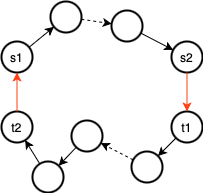
\includegraphics[scale=0.5]{skizze_reduktion.png}
	
	$f$ ist offensichtlich total. Außerdem lässt sich eine DTM konstruieren, die $f$ in polynomieller Laufzeit berechnet:
	\begin{itemize}
		\item Syntaxcheck, ob $w=c(V,E,s_1,s_2,t_1,t_2)$ mit einem Graph $G=(V,E)$ und $s_1,s_2,t_1,t_2 \in V$ (in $O(|V|+|E|)=O(n)$)
		\item Passendes zusammensetzen der Ausgabe zu $c(V,E\cup \{(s_2,t_1),(t_2,s_1)\},(s_2,t_1),(t_2,s_1))$ (in $O(1)$)
	\end{itemize}

	Es bleibt noch zu zeigen, dass $w \in 2VDP \Leftrightarrow f(w) \in SC$ gilt. Dies beweisen folgende Äquivalenzumformungen ($\forall w \in \Sigma^*$):
	\begin{align*}
		w \in 2VDP \Longleftrightarrow\ &w=c(V,E,s_1,s_2,t_1,t_2)\ mit\ Graph\ G=(V,E)\ und\ s_1,s_2,t_1,t_2 \in V\\
		&\wedge\ \exists\ Pfade\ p_1=s_1...s_2\ und\ p_2=t_1...t_2\ in\ G: \forall\ u \in p_1,\ v \in p_2: u\neq v\\
		\Leftrightarrow\ &f(w)=c(V,E\cup \{(s_2,t_1),(t_2,s_1)\}=E',(s_2,t_1),(t_2,s_1))\ mit\ Graph\\
		&\ G'=(V,E')\ und\ s_1,s_2,t_1,t_2 \in V\ \wedge\ \exists\ Pfade\ p_1=s_1...s_2\ und\ p_2=t_1...t_2\ in\ G':\\
		&\ \forall\ u \in p_1,\ v \in p_2: u\neq v\\
		\Leftrightarrow\ &f(w)=c(V,E',(s_2,t_1),(t_2,s_1))\ mit\ Graph\ G'=(V,E')\ und\ (s_2,t_1),(t_2,s_1) \in E'\\
		&\ \wedge\ \exists\ Pfad\ p=s_1...s_2t_1...t_2s_1\ in\ G':\ \forall\ n,m \leq k:=|p| : p_n\neq p_m,\ außer\ p_1=p_k \\
		\Leftrightarrow\ &f(w) \in SC
	\end{align*}
	\textit{Informelle Beschreibung: Zusammensetzen der zwei knoten-disjunkten Pfade über zwei neue Kanten, die jeweils die Endpunkte verbinden, zu einem einfachen Kreis.}

	Somit gilt $2VDP \leq_p SC$ und da $2VDP$ NP-vollständig ist,  muss $SC$ NP-hart sein.
	
	Um noch zu zeigen, dass $SC$ in NP liegt, muss eine NTM skizziert werden, die $SC$ in polynomieller Zeit entscheidet:
	\begin{enumerate}
		\item Starte mit einem leeren Pfad durch den Graphen ($O(1)$).
		\item Rate nun aus den vom letzten Knoten aus erreichbaren Knoten, die noch nicht im Pfad vorkommen (außer dem Startknoten), nichtdeterministisch den nächsten Knoten des Pfades, sodass am Ende (falls dieser existiert) ein Simple Circle gefunden wird ($O(n)$).
		\item Wiederhole den vorherigen Schritt solange, bis der Startknoten wieder erreicht wird - in diesem Fall wurde eine Lösung gefunden $\Rightarrow$ halten und akzeptieren - oder keine weiteren Knoten hinzugefügt werden können - in diesem Fall gibt es keine Lösung $\Rightarrow$ halten und nicht akzeptieren ($O(n)$).
	\end{enumerate}

	Es folgt, dass $SC$ in NP liegt und somit NP-vollständig ist.

	\item 
	Folgender Algorithmus löst USC:
	\begin{enumerate}
		\item Überprüfe, ob $e_1 = e_2$.
		\item Falls $e_1 = e_2$ und $e_1=(e_1',e_1''),\ e_2=(e_2',e_2'')$ starte A unter Eingabe $e_1',e_1'',e_2'',e_2'$ \begin{itemize}
			\item Falls A eine Lösung ausgibt, ist der Pfad $p=p_1\circ p_2$ eine Lösung von USC
			\item Falls A keine Lösung findet, gibt es auch für USC keine Lösung
		\end{itemize}
		\item Falls $e_1 \neq  e_2$ und $e_1=(e_1',e_1''),\ e_2=(e_2',e_2'')$ starte A unter Eingabe $e_1'',e_2'',e_2',e_1'$ \begin{itemize}
			\item Falls A eine Lösung ausgibt, ist der Pfad $p=p_1\circ e_2'e_2''\circ p_2\circ e_1'e_1''$ eine Lösung von USC
			\item Falls A keine Lösung findet, gibt es auch für USC keine Lösung
		\end{itemize}
	\end{enumerate}
	\textit{Anmerkung: $\circ $ meint hier die Aneinanderreihung oder Konkatenation von Pfaden. Dabei werden die Knoten in den Pfaden zusammen hintereinander geschrieben, wobei der letzte Knoten des ersten Pfades mit dem ersten Knoten des zweiten Pfades übereinstimmen muss und nur einmal nidergeschrieben wird. Bsp.: $abc\circ cde=abcde,\ \forall a,b,c,d,e \in V$.}

	\textbf{Laufzeitanalyse:}\\
	Die Überprüfung in Schritt 1, das Starten von A sowie die Überprüfung und Rückgabe in Schritt 2 und 3 laufen jeweils in $O(1)$. Der Durchlauf von A in Schritt 2 und 3 hat höchstens eine polynomielle Laufzeit in der Größe der Eingabe, da U2VDP in $\mathcal{P}$ liegt.\\
	Somit hat der beschriebene Algorithus insgesamt höchstens eine polynomielle Laufzeit in der Größe der Eingabe.

	Folglich liegt USC in $\mathcal{P}$.

\end{teile}
